\section{State estimation and Observabilty}

\noindent
Let us consider the LTI system (without input):
\begin{align*}
    &x(k+1)=Ax(k)\\
    &y(k)=Cx(k)
\end{align*}

\noindent
$y(k)\in \mathbb{R}^q$, $x(k) \in \mathbb{R}^n$, $A\in\mathbb{R}^{n,n}$, $C\in\mathbb{R}^{q,n}$\\

\noindent
The \textbf{State estimation} is the procedure by which we can \textbf{recover} the state $x(k)\in\mathbb{R}^n$ of the system from measurements $y(k)$ for $k=0, 1, 2, ...$. \textbf{Note that...} every element of the vector $y(k)$ is a measure from a sensor, and so we have $y_i(k)\in\mathbb{R}$.\\
We can say that a system is \textbf{Observable} if exists a finite time $T\in\{0,1,...\}$ such that \textbf{$x(0)$} can be recovered from the measurements $y(k), \quad k=0,1, ..., T-1$. \\

\noindent
But why only $x(0)$? Let us compute $y(0), ..., y(T-1)$ to verify this fact: 
\begin{flalign*}
&y(0)=Cx(0)
\\&y(1)=Cx(1)=CAx(0)
\\&y(2)=Cx(2)=CA^2x(0)
\\&...
\\&y(T-1)=...=CA^{T-1}x(0)
\end{flalign*}
At this point by using the vectorial notation, we have:
\begin{equation*}
    \begin{pmatrix} y(0)\\ y(1)\\ y(2)\\   \vdots\\    y(T-1) \end{pmatrix} 
    =
    \begin{pmatrix}
        C\\ CA \\ CA^2 \\ \vdots \\ CA^{T-1} 
    \end{pmatrix} x(0)
\end{equation*}

$\mathcal{O}_T$ = 
$\begin{pmatrix}
    C\\ CA \\ CA^2 \\ \vdots \\ CA^{T-1} 
\end{pmatrix}$ 

$\in\mathbb{R}^{qT, n}$ where if $T=n$ we call 
$ \mathcal{O}_n$ 
the \textbf{Observability matrix}.\\
\noindent
When the equation 
\begin{equation*}
    \begin{pmatrix} y(0)\\ y(1)\\ y(2)\\   \vdots\\    y(T-1) \end{pmatrix}= \mathcal{O}_T  x(0) 
\end{equation*}
has a \textbf{unique solution} the system is observable.
At this point, we distinguish two different cases: 
\begin{itemize}
    \setlength\itemsep{0em}
    \item $qt<N$ the system is \textit{underdetermined}
    \item $qt\geq N$ and $rank(\mathcal{O}_T)=n$, then we can (pseudo)invert it. In particular if  $qT=n$ then $$x(0)=\mathcal{O}_T^{-1}y(k)$$ otherwise if $qT>n$ then $$x(0)=(\mathcal{O}_T^T\mathcal{O}_T)^{-1}\mathcal{O}_T^Ty(k)$$
\end{itemize}
Where we call \textbf{Moore-Penrose pseudoinverse} the matrix 
    $\mathcal{O}_T^{\dagger}=(\mathcal{O}_T^T\mathcal{O}_T)^{-1}\mathcal{O}_T^T$

\begin{theorem}{(Kalman, 1960)}
    An LTI system is observable if and only if rank($\mathcal{O}_n$)=n
\end{theorem}
In general there are two approaches for the state estimation: 
\begin{itemize}
    \setlength\itemsep{0em}
    \item \textbf{static approach}: solving the equation like we have just seen.
    \item \textbf{dynamic approach}: by using a \textbf{Luemberger Observer} that allow us to recover the state after a bunch of steps. 
\end{itemize}

\section{Secure state estimation}
\noindent
In this section we make a try to expand the concept of \textbf{Observability and state estimation} when we have attacks on the sensors, and so the additive term $a(k)$ in the output equation.
\begin{align*}
    &x(k+1)=Ax(k) \\
    &y(k)=Cx(k)+a(k)
\end{align*}
\textbf{Assumption} The term $a(k)\in\mathbb{R}^q$ is  {\color{red}\textbf{sparse}} in the sense that no more than $h\ll q$ of its elements are non-zero. By using the $l_0$-norm, $\lVert a\rVert_0\le h$. \\

We refer to \textbf{Secure state estimation} when we want recover the state $x(0)$ from sensors' measurements $y(k), k=0,1,...$ and \textbf{unknown attacks} $a(k)$. (As we said we are not able to model attacks in a proper way, we wouldn't have a different theory and several techniques to face the problems related to them).

Let us anylize the mentioned problem by spotting the differences that occurs in the case of attacks: 
\begin{flalign*}
&y(0)=Cx(0)+a(0)
\\&y(1)=Cx(1)=CAx(0)+a(1)
\\&y(2)=Cx(2)=CA^2x(0)+a(2)
\\&...
\\&y(T-1)=...=CA^{T-1}x(0)+a(T-1)
\end{flalign*}
Then 
\begin{equation*}
    \begin{pmatrix} y(0)\\ y(1)\\ y(2)\\   \vdots\\    y(T-1) \end{pmatrix} 
    =
    \begin{pmatrix}
        C\\ CA \\ CA^2 \\ \vdots \\ CA^{T-1} 
    \end{pmatrix} x(0) + 
     \begin{pmatrix} a(0)\\ a(1)\\ a(2)\\   \vdots\\    a(T-1) \end{pmatrix} 
\end{equation*}
where we have {\color{red}qT equations} for {\color{red}$n+qT$ unknowns}! That would indicate potentially \textbf{infinitely many solutions}.\\
{\color{blue}Despite this observation if we add the hypotesis that the vector containing the attack is \textbf{sparse}, in some situations we could have a unique solution to this problem. 
}
\begin{lemma}
    \large{
    We say that $h$ errors are \textbf{correctable} after T steps if its possible to recover any $x(0)$ given $y(0), ..., y(T-1)$ under the condition $\lVert a \rVert_0 \le h$, for each $k=0,..., T-1$}.
\end{lemma}
This corresponds to ask that the problem \\

\hspace*{-5mm}
\begin{tikzpicture}
\node [mybox] (box){%
    \begin{minipage}{.96\textwidth}     %Larghezza del box
           \begin{equation*}
    \begin{pmatrix} y(0)\\ y(1)\\ y(2)\\   \vdots\\    y(T-1) \end{pmatrix} 
    =
    \begin{pmatrix}
        C\\ CA \\ CA^2 \\ \vdots \\ CA^{T-1} 
    \end{pmatrix} x(0) + 
     \begin{pmatrix} a(0)\\ a(1)\\ a(2)\\   \vdots\\    a(T-1) \end{pmatrix} 
     \quad \textrm{s.t.} \quad  \lVert a \rVert_0 \le h,  k=0,..., T-1
\end{equation*}
    \end{minipage}
};
\end{tikzpicture}%


\noindent
had a \textbf{unique solution}.



\noindent
Now we have to face with two problems: 
\begin{enumerate}  
    \setlength\itemsep{0em}
    \item Under \textbf{which conditions} can I solve the proposed problem?
    \item \textbf{How can I solve} it?
\end{enumerate}

\noindent
\section{Well-Position of the problem (Static case)}
Let us analyze the problem in a very particular case, that is when the system we want to ovbserve is \textbf{static}. That is the matrix $A\in \mathbb{R}^{n,n}$ is the identity matrix $\mathbb{I}_n$. This corresponds to state that $x(k+1)=x(k)=x$ (remember that we have no input $u(t)$).\\
In this case the observability matrix has a very simple form, in particular it is equal to the matrix $C\in\mathbb{R}^{q,n}$. We have that the problem becomes: 
{   \large{
    $$y=Cx+a \quad \textrm{s.t.} \quad \lVert a \rVert_{0} \le h$$ }
}

\noindent
It is useful to give these formal definitions:\\
\begin{lemma}[h-sparsity]
    A vector is said to be \textbf{h-sparse}, if  $\lVert a \rVert_0 = h  $
\end{lemma}

\begin{lemma}[Support]
    Given $a\in \mathbb{R}^q$ we denote with $Supp(a)=\{i: a_i \ne 0\}$, the set of i such that the i-th component of the vector is a non-zero number.
\end{lemma}

\noindent
{\color{red} \textbf{How the attack could be done in order to not to be 'detectable'?}}
 Let's consider an $a=Cw, \quad w \in \mathbb{R}^n, w \ne 0$ and assume it is that $\lVert Cw \rVert_0 \le h$ (for the assumption we made). We sobstitute in the equation and obtain:
$$y=Cx+Cw=C(x+w) \quad \textrm{s.t.} \quad \lVert Cw \rVert_0 \le h$$
Actually, if such $w$ exixts, the \textbf{attack is feasible} and so not detectable. This property depends strongly on the property of the matrix $C$.\\
Fortunately we have a \textbf{proposition} that provide us with an equivalence to determine the \textbf{resilience} of the system to h  attacks.


\vspace{0.3cm}

 \hspace*{0mm}
\begin{tikzpicture}
\node [mybox] (box){%
    \begin{minipage}{.96\textwidth}
          \begin{proposition}[Correctability]
    \large{
    h errors are correctable (or equivalently \textbf{the system is resilient against h attacks)} after T steps if and only if for all $z\in\mathbb{R}^n$, $\lVert \mathcal{O}_Tz \rVert_0 > 2h$.}
    $$\textrm{\textbf{System correctable}} \quad \Longleftrightarrow \quad \forall z \in \mathbb{R}^n , \quad \lVert \mathcal{O}_Tz \rVert_0>2h$$
\end{proposition}
    \end{minipage}
};
\end{tikzpicture}%

\noindent
In the static case the Proposition 1 becomes: $$\textrm{\textbf{System correctable}} \quad \Longleftrightarrow \quad \forall z \in \mathbb{R}^n , \quad \lVert Cz \rVert_0>2h$$
\begin{proof}
    As this is a characterization property we have to proof the proposition in the two direction $\Leftarrow$ and $\Rightarrow$. We give this proof for the static case, but the procedure for the more general case is analogue.
    \begin{itemize}
        \item {\Large{\textbf{[Proof of $\Leftarrow$] }}}
        {\color{blue} Assuming that 
        $\forall z \in \mathbb{R}^n$ we have $\lVert Cz \rVert_0 > 2h $ we want to demonstrate that h errors are correctable}, that is the problem has a unique solution.  As in many situation we want to demonstrate the uniqueness of something, we can go on \textbf{by contraddiction}. In particular assume that $y=Cx+a$ s.t. $\lVert a \rVert_0 \le h$ has got two different solutions: 
        $$\begin{pmatrix}
            x'\\ a'
        \end{pmatrix} and \begin{pmatrix}
            x''\\a''
        \end{pmatrix}$$

        then we have that $y=Cx'+a' \quad \textrm{s.t.} \quad \lVert a' \rVert_0 \le h$ but also $y=Cx''+a'' \quad s.t. \quad \lVert a'' \rVert_0 \le h $. $Cx'+a'=Cx''+a''$ $\Longleftrightarrow C(x'-x'')=a''-a'$ But due to the fact that $a'$ and $a''$ are h-sparse we can obtain by substracting them a vector which is \textbf{at most} 2h-sparse. 
        We have finished because we found a contradiction , that is, $\exists  z \in \mathbb{R}^n, \lVert Cz \rVert_0 \le 2h$. In this case $w=a'-a''$
        
        \item {\Large{\textbf{[Proof of $\Rightarrow$] }}}{\color{blue} Assuming that h errors are correctable,  we want to demonstrate that 
        $\forall z \in \mathbb{R}^n$ we have $\lVert Cz \rVert_0 > 2h $ }. Similarly the former case,  we can demonstrate the property by contradiction assuming that $\exists w \in \mathbb{R}^n \quad \lVert Cw \rVert_0 \le 2h$. We can write such $Cw$ like a sum of two (at most) h-sparse vectors $g_1$ and $g_2 \rightarrow Cw=g1+g2$. But we can also say that $Cw=g_1+g_2 \longleftrightarrow Cw-g_1=g_2=C 0+g_2 $. In this way we are saying that we have \textbf{two distinct solutions}, this is in contradiction with our hypotesis. \texttt{QED}
    \end{itemize}
\end{proof}

\noindent
The proposition that has just been proved is very powerful, but how are we able to try for all $z$ that the statement is valid? In the great majority of the situations is easier to provide a \textbf{counter-example}.\\
Now we are going to do some example and then to provide (at least) a necessary condition for well-position of the problem of correctability. 

\subsection{Some examples}
{\color{orange}\subsubsection{Example 0: a "naive" example}}
Consider that we have $C=\mathbb{I}_n$, $q=n$, $h=1$, $n=3$. In this case the output equation is: 
\begin{align*}
    &y_1=x_1\\
    &y_2=x_2\\
    &y_3=x_3
\end{align*}
As we can see the system is \textbf{perfectly observable} because each measurement of $y$ gives an element of the state, but suppose that we know that there is an attack ($h=1$), but we don't know where. If one of the measurement is corrupted, there is no way to recover the state of the system $\Rightarrow$ $C$ is not correcting h errors $\Rightarrow$ the system is not resilient to h attacks. In an intuitive way we can say that we could add more sensors to improve the situation, it is 'the path' that follows the next example.

{\color{orange}\subsubsection{Example 1: add more sensors (increase q)}}
At this point we change the (sensing) matrix $C$ by adding new measurements, so
$$C=\begin{pmatrix}
    1 &0 &0\\0& 1& 0\\0& 0 &1 \\ 1& 0& 0 \\ 0& 1& 0
\end{pmatrix}$$
What has changed here is that we have \textbf{two more }sensors. We have a duplication of $C_1$ and $C_2$ (we indicate with $C_i$ the i-th row of C). If $y_1=C_1x=y_4=C_4x$ and $y_2=C_2x=y_5=C_5x$ than we can state that the attack is on the sensor 3. But\textbf{ what if either $y_1 \ne y_4$ or $y_2 \ne y_5$}? We have no way to know which sensor has been attacked. If I switched off this couple of devices I can't observe anymore one of the component of the state vector. \\
This was only an \textbf{intuitive way} to understand this fact. How can we formalize it? 
We can say that the couple $(C_1, C_2)$ has a \textbf{non trivial kernel}. That is the equation:
$$\begin{pmatrix}
    1&0&0\\0&1&0
\end{pmatrix}z=\begin{pmatrix}
    0\\0
\end{pmatrix}$$
has a non zero solution. In particular a solution could be $z=\begin{pmatrix}
    0\\0\\\alpha
\end{pmatrix}$ such $z$ produces 
$$Cz=\begin{pmatrix}
    0\\0\\\alpha\\0\\0
\end{pmatrix} \quad \alpha \in \mathbb{R}$$ which due to the fact which is 1-sparse, is \textbf{in contradiction} with the proposition.\\
Conclusion: \textbf{even this matrix does not correct h=1 error $\Rightarrow$ the system \textbf{is not} resilient}!

{\color{orange}\subsubsection{Example 2: more mixed measurements}}
Freezing the other parameters, let us change again the matrix $C$ in the following way: 
$$C=\begin{pmatrix}
    1&0&0\\0&1&0\\0&0&1\\1&1&1\\1&-1&1
\end{pmatrix}$$
It is quite clear that there is a triple of rows of C which are linearly dependent, specifically $C_5=C_4-2C_2 \Rightarrow$ the triple has a non trivial kernel. By doing simple algebraic steps we desume that a solution could be  $z=\begin{pmatrix} 
    \alpha\\0\\-\alpha
\end{pmatrix}$ which generates a 2-sparse $Cz$ we have again a contradiction! Conclusion: \textbf{C is not resilient}. 

{\color{orange}\subsubsection{Example 3: linearly independent measurements}}
Now we provide the following $C$ matrix: 
$$C=\begin{pmatrix}
    &1&0&0\\&0&1&0\\&0&0&1\\&1&1&1\\&1&2&-1
\end{pmatrix}$$
In this case all the triples are linearly independent, this cause the relative kernel to be trivial $\rightarrow$ there is no way to produce a counter-example. 
Conclusion: this  $C$ matrix corrects h=1 error.

\subsection{A necessary condition for well-position}
Let $C\in \mathbb{R}^{q,n}$, $rank(C)=n$ and $q>n$, it is quite clear that any subset $\Omega$ composed by $n-1$ rows  has got a non trivial kernel. This implicates that the sparsity is not larger than $q-(n-1)$, that is $2h < q-(n-1)$ or equivalently $h \le q-n$. From which I can recover the following inequality: $$q\ge 2h+n$$
It is immediate to understand that if I want to correct $h=1$ error with $n=3$, we need at least of $q=5$ sensors.

This fact bring us to state that: 
\begin{itemize}
    \item Large $q$ is not sufficient for \textbf{resilience} 
    \item On the other hand there is a \textbf{minimum q} which I need to correct a certain number $h$ of errors.
\end{itemize}

\section{Reformulation of $y=Cx+a \quad \textrm{s.t.} \quad    \lVert a \rVert_0 \le h$}
\noindent
The second question to answer is: \\
{\begin{center}
\textbf{
    How can we solve the problem $y=Cx+a \quad \textrm{s.t.} \quad    \lVert a \rVert_0 \le h$?}
\end{center}} 
The problem can be reformulated as follows:
{   \large{
        $$\min_{x\in\mathbb{R}^n, a\in\mathbb{R}^q} \lVert a \rVert_0 \quad \textrm{s.t.} \quad y=Cx+a$$
    }
}\\
It can be proved that \textbf{if the system is resilient to h attacks the solution to this problem corrects h errors}. Unfortunately, even this form of the problem has its drawbacks: 
\begin{itemize}
    \item As the problem is a combinatorial one, is \textbf{not feasible} (NP-Hard)
    \item The \textbf{objective function} which contains an $\ell_0$ norm is \textbf{not convex, non continuous and non differentiable in 0}
\end{itemize}
The solution is going in the direction of \textbf{convex relaxation}: 
\begin{enumerate}
    \item In the objective function, we choose to relax $\lVert a \rVert_0$ with its \textbf{best CONVEX approximation} $\lVert a \rVert_1$; it is \textsc{Convex}, \textsc{Continuous} but \textsc{Non differentiable in 0} (we can face this problem);
    \item In the real world, we must take into account the noise that could appear in the equation $y=Cx+a$ and so it becomes $y\approx Cx+a$, this leads to the \textbf{Least Squares (LS) problem} $$\min{ \frac{1}{2}\lVert y-Cx-a \rVert_2^2}= 
    \min{\frac{1}{2}\Bigg\lVert y - \begin{pmatrix}
        C & I 
    \end{pmatrix}\begin{pmatrix}
        x\\
        a
    \end{pmatrix} \Bigg\rVert}$$ 
\end{enumerate}

Combining this two approximations, due to the fact we want to minimize both the terms, the \textbf{resulting problem to solve} is: 

\hspace*{-5mm}
\begin{center}
    \begin{tikzpicture}
    \node [mybox] (box){%
        \begin{minipage}{.80\textwidth}
                %Qui testo
                {
                \color{black}
                \Large{
                    $$
                    \min_{x\in\mathbb{R}^n, a\in\mathbb{R}^q}{\frac{1}{2}\Bigg\lVert y - \begin{pmatrix}
                        C & I 
                    \end{pmatrix}\begin{pmatrix}
                        x\\
                        a
                    \end{pmatrix} \Bigg\rVert}+\lambda\lVert a \rVert_1, \quad \lambda>0
                    $$
                }}
                
        \end{minipage}
    };
    \end{tikzpicture}%
\end{center}



\subsection{Why $\ell_1$-regularization promotes sparsity?}
\begin{figure}[h]
    \centering
    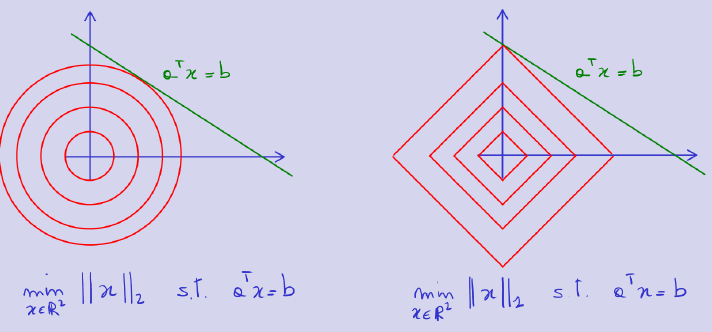
\includegraphics[scale=0.8]{images/Sparsity.png}
    \caption{$\ell_p$-norms and sparsification}
    \label{fig:enter-label}
\end{figure}
In the approximation we have just made, we have considered the $\ell_1$-norm. But why it is the best we could do? Let us consider to solve the problem $$\min_{x\in\mathbb{R}^2} \lVert x \rVert_2 \quad  \textrm{s.t.} \quad a^Tx=b$$ 
The term $\lVert x \rVert_2=k, k\in\mathbb{R}$ is a circle in the plane. We start from $k=0$, and we increase it until we reach the line to satisfy the (linear) constraint. The solution we obtain is certainly not sparse because it is of the form $x^*=(x_1^*, x_2^*)$ both non-zero real number.\\
\noindent
On the other hand if we consider the problem: 
$$\min_{x\in\mathbb{R}^2} \lVert x \rVert_1 \quad  \textrm{s.t.} \quad a^Tx=b$$ 
we note that the solution we can find (by using the same method as before) is sparse. We have seen in an intuitive way that $\ell_2$-norm takes the components of the solution close to zero in a "democratic way", in other words without 'reset' any component. At the opposite the $\ell_1$-norm push to zero \textbf{only some components} making a selection among them $\longleftrightarrow $ this promotes \textbf{"sparsification"}.\\

\noindent
{
    \color{blue}
    [Note that we have just showed a trivial way to understand why we have chose one regularization instead of another. The topic would require a more accurate and rigorous explanation, which we don't care.]
}

\subsection{Some observations}

\subsubsection{The problem has a connection with LASSO}
The problem we found to solve after applying \textbf{relaxation} is very similar to the problem of \textbf{LASSO} (Least Absolute Shrinking and Selection Operator) in fact in its original formulation we have: 
$$\min_{x\in\mathbb{R}^n} \frac{1}{2}\lVert Ax-y \rVert_2^2+\lambda\lVert x \rVert_1$$
but this give an entire sparse solution. In our problem only a piece of the solution is sparse, whose linked to attacks $a$, so we can see our problem as a "\textbf{Partial LASSO}" because we have \textbf{no regularization} on the term $x$ of the solution $\begin{pmatrix}
    x\\a
\end{pmatrix}$.

\subsubsection{The problem has a connection with "Compressed Sensing"}
The problem
 $$
    \min_{x\in\mathbb{R}^n, a\in\mathbb{R}^q}{\frac{1}{2}\Bigg\lVert y - G\begin{pmatrix}
        x\\
        a
    \end{pmatrix} \Bigg\rVert}+\lambda\lVert a \rVert_1, \quad \lambda>0,
    \quad 
    G=\begin{pmatrix}
        C & I 
    \end{pmatrix}
    $$
as the $G$ matrix has more columns than rows, is a \textbf{fat matrix} and without regularization the problem has infinitely many solutions. We can consider the $y$ a \textbf{linear compressed measurement} vector.
The problem of \textbf{recover a sparse vector from compressed linear measurement} has a strong connection with the \textsc{Compressed sensing} problem. Also here we have a \textbf{"Partial Compressed Sensing"} as only a part of the solution is sparse.\\

\noindent
{
\large{
    \color{red}
    After a "long journey" we have understood that for the \textbf{secure state estimation of CPS under adversarial attacks} we have to solve a \textbf{Partial LASSO} problem. For this reason we seek a way to solve it $\Rightarrow$ Iterative Algorithms
    }
}
    
\section{IST: an algorithm for LASSO}
\noindent
{\color{blue}
\textit{
    \textbf{Premise} In this course we will not see any black box technique, we will go through the direction of \textbf{iterative algorithms} to solve the LASSO problem.\\
    \noindent
    In the framework of \textbf{Convex Optimization} one of the most used algorithms (also in Data Science/Machine Learning...) is the \textbf{Gradient Descent Algorithm}. But in the LASSO we have a $\ell_1$-regularization, which is not differentiable in 0. We can't even avoid to consider it because we want to reach the (global) \textbf{minima}. We wonder if using an approximation could be the solution (eg. \textbf{subgradients}), however again this not produce a \textit{sparse solution}. 
}\\
}

\noindent
Once the proper promises have been done, we can introduce this algorithm for solving the \textbf{(sparse) optimization problem} of LASSO. 
The algorithm is called \textbf{Iterative Shrinkage/Thresholding (IST)} and it is a variant of the \textit{Descent Gradient Algorithm}. After the definition and a general description, we are goingo to list the steps of the algorithm itself. Initially we consider the original LASSO problem
$$\min_{x\in\mathbb{R}^n} \frac{1}{2}\lVert Ax-y \rVert_2^2+\lambda\lVert x \rVert_1$$ in which we call $F(x)=\lVert Ax-y \rVert_2^2$ the Least-Squares functional. Moreover we know that $\nabla F(x) = A^T(Ax-y)$.\\

\noindent
\textbf{Definition (Shrinkage/Thresholding operator)} The \textbf{Shrinkage/Thresholding operator} $\mathbb{S}_{\alpha}$ is a component wise operator $\mathbb{S}_{\alpha}: \mathbb{R}^p \rightarrow \mathbb{R}^p, \alpha >0$. For any $x_i\in \mathbb{R}$:
\begin{equation*}
    \mathbb{S}_{\alpha}(x_i) =
        \begin{cases}
            x_i-\alpha & \text{if $x_i$>$\alpha$} \\
            x_i+\alpha & \text{if $x_i$ < -$\alpha$}\\
            0 & \text{if $ \lvert x_i \rvert \le \alpha$}\\ 
        \end{cases}
\end{equation*}



\hspace*{-5mm}
\begin{tikzpicture}
\node [mybox] (box){%
    \begin{minipage}{.96\textwidth}

    \textbf{\Large{IST Algorithm}}\\
        \begin{enumerate}
            \item Initialization: $x_0\in\mathbb{R}^p$, e.g. $x_0=0$
            \item For $k=0,..., T_{max}$
            \Large{
            \begin{equation*}
                x(k+1)=\mathbb{S}_{\lambda \tau} \left[ x(k)-\tau\nabla F(x(k))
                \right]
            \end{equation*}
            }
        \end{enumerate}
    \end{minipage}
};
\end{tikzpicture}%

\vspace{0.5cm}
\noindent
The parameter $\tau$ has to be "small enough" so that the algorithm works as desidered. It has been demonstrated that the algorithm converge to the minimum of the LASSO functional $\frac{1}{2}\lVert Ax-y \rVert_2^2+\lambda\lVert x \rVert_1$. The \textbf{iterative nature} and simplicity of this method, makes it adaptable also for: \textbf{dynamic} and \textbf{distributed} systems.

\subsection{Derivation of IST Algorithm} 
Let us do a quick RECAP of the latest notions we introduced...\\
Generally speaking, when we have some measurements $y=A\tilde{x}+\eta$ where $\tilde{x}$ is the \textbf{true vector} to recover, we are able to find an \textbf{estimate} of it by solving the problem 
$$x^{*} = \textrm{arg} \min_{x\in \mathbb{R}^n} \frac{1}{2}\lVert y-Ax \rVert_{2}^{2}$$
also known as the \textbf{Least Squares (LS)} problem, where the obtained $x^*$ is the estimate of the true vector. How can we solve this problem?\\
The \textbf{Gradient Descent} method is one of the most used in this field to retrieve a solution for LS problem. This algorithm step by step proceeds in the direction of the gradient, moving from the previous point of a \textbf{step size} called $\tau$ (small enough). Then we have 
\begin{equation} 
\label{eq:1}
    x(k+1)=x(k)-\tau \nabla{F(x)}, \quad F(x)= \lVert y-Ax \rVert_2^{2} \quad \textrm{(LS functional)}
\end{equation}
 for $k=0,1, 2, ....$  \\
We can observe that the expression (\ref{eq:1}) is a Discrete Time Linear Time Invariant System (DT LTI), therefore we can study its properties by using the known results from the Theory.\\

Differently from the case which has just mentioned, in the LASSO problem we have the {$\ell_1$-norm} too, because we are interested in finding a \textbf{sparse solution} (in our framework of \textbf{CPS under adversarial attacks} this is an important requirement). It is good to remind that the LASSO is a \textbf{convex, non-differentiable} problem. \\
Then, how can we solve it? Its solution can be retrieved by using any convex optimization solver (\texttt{cvx,lasso, ...}). On the other hand, the \textit{Gradient Descent} algorithm is not effective! (Gradient of a non differentiable functional?? We can't!). Our \textbf{approach} is using the \textbf{ISTA} Algorithm of which it is given a \textbf{possible interpretation}. \\

Let the functional $F(x)=\frac{1}{2}\lVert y-Ax \rVert_{2}^{2}+\lambda\lVert x \rVert_1$ be the LASSO functional. We define now a \textbf{surrogate functional} which will guide our \textit{derivation of ISTA} as 
\begin{equation}    \label{eq:SurrogateFunctional}
    \mathcal{R}(x,b)=F(x)+\frac{1}{2\tau}\lVert x-b \rVert_2^2 -\frac{1}{2} \lVert Ax-Ab \rVert_2^2,
    \quad \tau > 0
\end{equation}
where $x$ is my 'standard' variable, while $b$ is an auxiliary variable. By using a little bit of linear algebra we note that:  
\begin{align*}
    &\frac{1}{2\tau}\lVert x-b \rVert_2^2 -\frac{1}{2} \lVert Ax-Ab \rVert_2^2 =
    \frac{1}{2\tau}\lVert x-b \rVert_2^2-\frac{1}{2} \lVert A \rVert_2^2 \lVert x-b \rVert_2^2=
    \frac{1}{2}  \bigg( \frac{1}{\tau} - \lVert A \rVert_2^2 \bigg) \lVert x-b \rVert_2^2
\end{align*}
and this quantity is non-negative if and only if $\frac{1}{\tau} > \lVert A \rVert_2^2 \Rightarrow \tau < \lVert A \rVert_2^{-2}$. This provides a guide to choose the $\tau$  and ensures that the \textbf{surrogate part} of the functional (\ref{eq:SurrogateFunctional}) is never negative, moreover it can immediately be noted that it is null if and only if $x=b \Rightarrow F(x)=R(x,x)$. That is the global minimum of $F(x)$ is the same of the global minimum of $R(x, x) \Rightarrow F(x^*)=R(x^*, x^*)$. At this point: our aim is to develop a \textbf{descent algorithm} for $F(x)$ which we will see that it is eased by $R(x, b)$.\\

It is not trivial to find a closed form for the solution of minimizing the surrogate functional considering both variables $x, b$ together. Therefore, we move in the direction of an \textbf{alternating minimization} (alternating $\Rightarrow$ in turn). This is both \textbf{feasible} and \textbf{leads to the minimum} of $F(x)$. More clearly:

$$\begin{cases}
    \min_{b\in \mathbb{R}^n } \mathcal{R}(x,b),& \quad \text{keeping $x$ as a constant} \\
    \min_{x \in \mathbb{R}^n} \mathcal{R}(x,b),&  \quad \text{keeping $b$ as a constant}
\end{cases}$$

\subsubsection{First step: minimizing with respect to $b$}
It is more trivial because we have seen recently that the \textit{surrogate part} depends on b, and it is minimum if $x=b$, then   
$$x=\textrm{arg}\min_{b \in \mathbb{R}^n} \mathcal{R}(x,b) $$

\subsubsection{Second step: minimizing with respect to $x$}
The problem here is find $\textrm{arg}\min_{x \in \mathbb{R}^n} \mathcal{R}(x,b)$. In this case we have to expand the functional by expressing the squared norm explicitly, to reach a conclusion. 
\begin{align}
\textrm{arg}\min_{x \in \mathbb{R}^n} \quad 
    &\mathcal{R}(x,b)=
    \textrm{arg}\min_{x \in \mathbb{R}^n} \quad 
    \frac{1}{2} \lVert Ax \rVert_2^2 +\frac{1}{2} \lVert y \rVert_2^2-yA^Tx+\lambda\lVert x \rVert_1+\\
    & \frac{1}{2\tau} \lVert x \rVert_2^2 + \frac{1}{2\tau} \lVert b \rVert_2^2-\frac{1}{\tau}b^Tx+\\
    &-\frac{1}{2}\lVert Ax \rVert_2^2 - \frac{1}{2}\lVert Ax \rVert_2^2 -b^TA^TAx = \\
    \label{eq: expanded}
    \textrm{arg}\min_{x \in \mathbb{R}^n} \quad 
    &\lambda \lVert x \rVert_1+\frac{1}{2\tau}\lVert x \rVert_2^2-x^T 
    \bigg( \frac{1}{\tau}b+A^Ty-A^TAb \bigg) =\\
    \label{eq:mult_tau}
    &\tau \lambda \lVert x \rVert_1 + \frac{1}{2} \lVert x \rVert_2^2 - x^T [b+\tau A^T(y-Ab)]+\frac{1}{2}\lVert b+\tau A^T(y-Ab) \rVert_2^2=\\
    \label{eq:final_step}
    \textrm{arg}\min_{x \in \mathbb{R}^n} \quad 
    &\tau\lambda\lVert x \rVert_1 + \frac{1}{2} \lVert x-q \rVert_2^2=
     \textrm{arg}\min_{x \in \mathbb{R}^n} \quad 
    \sum_{i=1}^{n} \bigg(\tau\lambda \lvert x_i \rvert + \frac{1}{2} (x_i-q_i)^2 \bigg)
\end{align}

In (\ref{eq:mult_tau}), by multiplying all terms in (\ref{eq: expanded}) by $\tau$ and by adding a constant term ${q= b+\tau A^T(y-Ab)}$ nothing change. Moreover the final step (\ref{eq:final_step}) is separable, in the sense that If I want minimize the sum, I can proceed \textbf{component wise}. Therefore

\begin{align}
     \textrm{arg}\min_{x \in \mathbb{R}^n} \quad 
    \sum_{i=1}^{n} \bigg(\tau\lambda \lvert x_i \rvert + \frac{1}{2} (x_i-q_i)^2 \bigg)
    &\Longleftrightarrow
     \textrm{arg}\min_{x_i \in \mathbb{R}} \quad
    \tau\lambda \lvert x_i \rvert + \frac{1}{2} (x_i-q_i)^2 = (...)=
\end{align}

\begin{equation}
    =\begin{cases}
        q_i-\tau\lambda &\quad \text{if}\quad q_i>\tau\lambda\\
        q_i+\tau\lambda\ &\quad \text{if}\quad q_i<-\tau\lambda\\
        0 &\quad \text{if}\quad q_i\in[-\tau\lambda, \tau\lambda]\\
    \end{cases}
\end{equation}
but this is the operator we formerly introduced as $\mathbb{S}_{\tau\lambda}(q)$ which pushes the component of the vector $q$ close to zero. We can reach a \textbf{conclusion}.\\
\noindent
Given $x_0=0$ for any $k=0,1,...$
\begin{enumerate}
    \item $b(k+1) =    \text{arg}\min_{b\in\mathbb{R}^n} \mathcal{R}(x(k),b)=x(k)$
    \item $x(k+1)=\text{arg}\min_{x\in\mathbb{R}^n} \mathcal{R}(x,b(k+1))=
    \text{arg}\min_{x\in\mathbb{R}^n} \mathcal{R}(x,x(k))=
    {\mathbb{S}_{\tau\lambda}[x(k)+\tau A^T(y-Ax(k))]}$
\end{enumerate}
Then, 
\begin{equation}\label{eq:ISTA_eq}
    x(k+1)={\mathbb{S}_{\tau\lambda}[x(k)+\tau A^T(y-Ax(k))]}
\end{equation}
which is our \textbf{Iterative Shrinkage/Thresholding algorithm (ISTA)}. Then, at the end of this discussion we have seen that the algorithm on which we focus comes from an \textbf{alternating minimization} of the surrogate functional $\mathcal{R}(x, b)$.\\

\hspace*{-5mm}
\begin{tikzpicture}
\node [mybox] (box){%
    \begin{minipage}{.96\textwidth}     %Larghezza del box
           \textbf{Theorem (1)} ISTA is a \textbf{descent algorithm} for LASSO, then $F(x(k+1))\le F(x(k))$
    \end{minipage}
};
\end{tikzpicture}

\textbf{Proof} The proof of the theorem above is very simple:
\begin{align*}
    F(x(k))=&\mathcal{R}(x(k), x(k))  \ge \quad &\text{(minimizing over x)} \\
    &\mathcal{R}(x(k+1), x(k))  \ge \quad &\text{(minimizing over b)}\\
    &\mathcal{R}(x(k+1), x(k+1)) = F(x(k+1),x(k+1))
\end{align*}

\hspace*{-5mm}
\begin{tikzpicture}
\node [mybox] (box){%
    \begin{minipage}{.96\textwidth}     %Larghezza del box
           \textbf{Theorem (2)} ISTA converges to the minimum of LASSO.
    \end{minipage}
};
\end{tikzpicture}

\subsection{Curiosity}
The equation (\ref{eq:ISTA_eq}) combines a linear part (the argument of the operator $\mathbb{S}$) and a \textbf{non linear part} that is the operator itself, being defined in a piece-wise fashion. The resulting system is a \textbf{Discrete Time Non Linear Time Invariant system} which is not trivial to treat.\\
This reminds a little the structure of a \textbf{neural network} where we have a \textbf{linear part} and a \textbf{non linear part} constituted by the \textbf{activating function}. For this reason the \textbf{evolution of ISTA} can be seen as a \textbf{Neural Network} application.

\subsection{Application of ISTA on CPS framework} 
We have seen recently that the problem of Cyber-Physical system under attacks can be formulated as follows: 
\begin{equation}
    \min_{x \in \mathbb{R}^n, a \in \mathbb{R}^q} 
    {\frac{1}{2} \bigg\lVert y-G \begin{pmatrix}
        x\\a
    \end{pmatrix} \bigg\rVert + \lambda \lVert a \rVert_1}
\end{equation}
that is a \textbf{partial LASSO} because only a part of the found solution is sparse, whose related to the (sparse) attacks. What about ISTA for Partial LASSO?
I have no limitations about the choice of the coefficient $\lambda$, in particular I can get $\lambda=0$ for the elements of the solution which are not interested by sparsity as it is the state of the system. Then, 
\begin{equation}
    \lambda\lVert a \rVert_1 = \lambda\bigg\lVert \begin{pmatrix}
        x\\a
    \end{pmatrix} \bigg\rVert_1 = 0\lvert x_1 \rvert+...+0\lvert x_n \rvert+
    \lambda \lvert a_1 \rvert + \lambda \lvert a_q \rvert
\end{equation}
This changes nothing, but it is essential that we made this variation in a way that the derivated descent algorithm could fit the "Partial LASSO" problem used for CPS purposes.
